\begin{apendicesenv}

\partapendices

\chapter{Questionário Gestão do Contrato}

\begin{figure}[H]
		\centering
			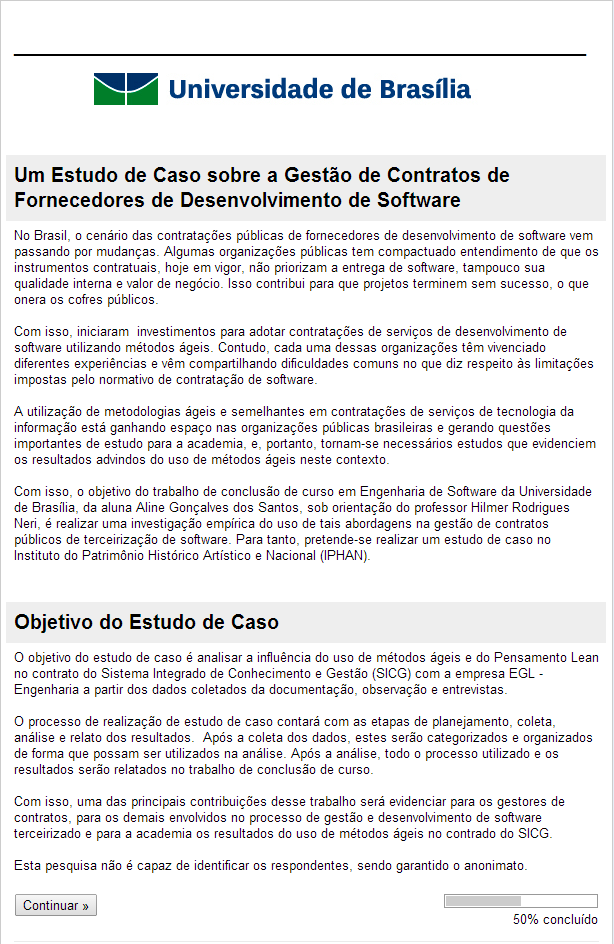
\includegraphics[scale=0.9]{figuras/quest1.png}

		\label{quest1}
\end{figure}

\begin{figure}[H]
		\centering
			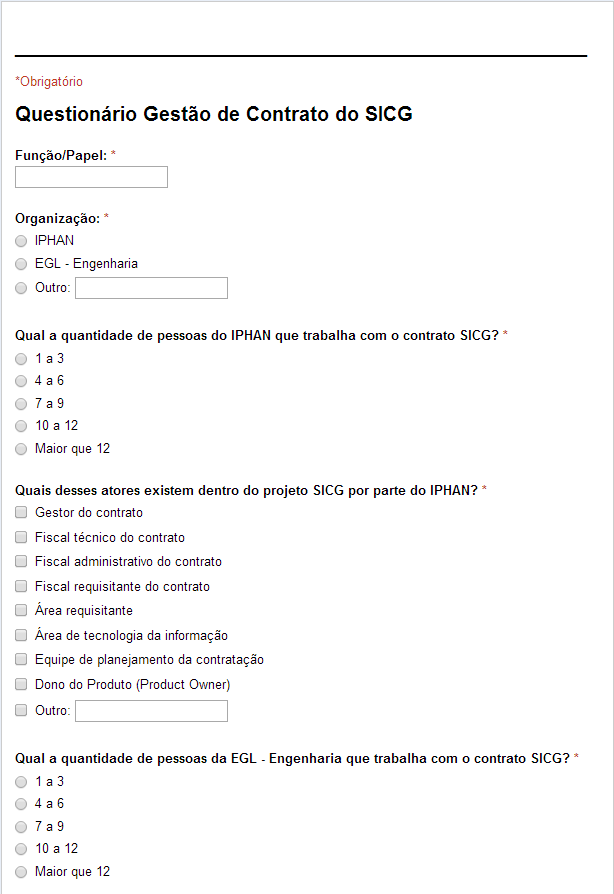
\includegraphics[scale=1.0]{figuras/quest2.png}

		\label{quest2}
\end{figure}

\begin{figure}[H]
		\centering
			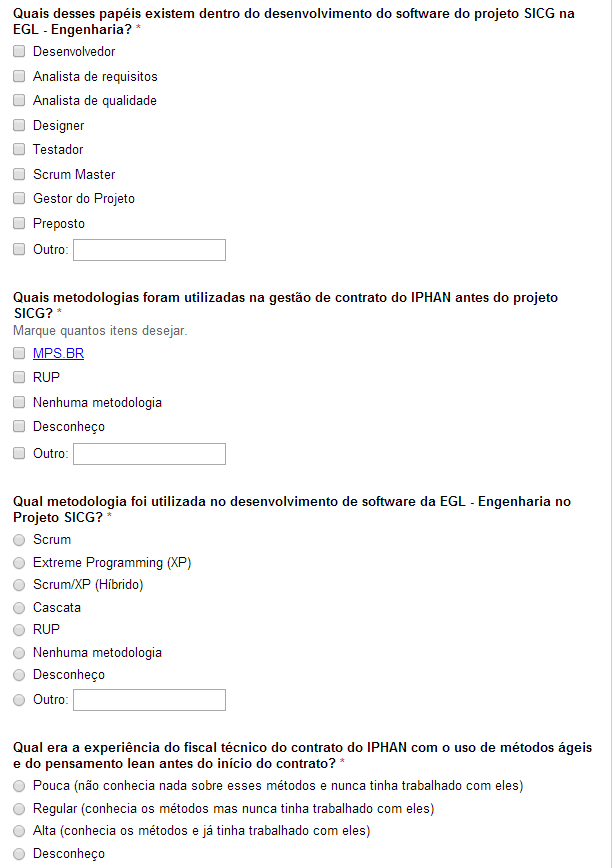
\includegraphics[scale=1.0]{figuras/quest3.png}

		\label{quest3}
\end{figure}

\begin{figure}[H]
		\centering
			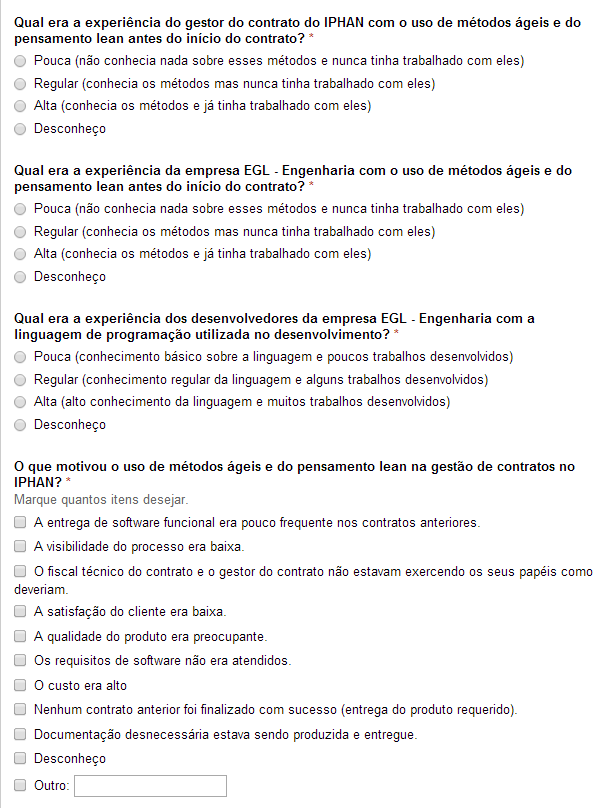
\includegraphics[scale=1.0]{figuras/quest4.png}

		\label{quest4}
\end{figure}

\begin{figure}[H]
		\centering
			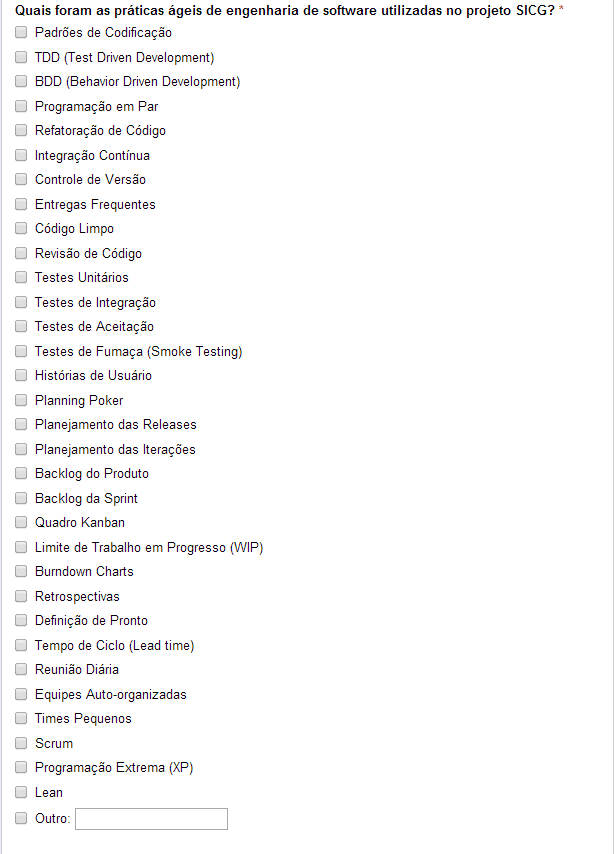
\includegraphics[scale=1.0]{figuras/quest5.png}

		\label{quest5}
\end{figure}

\begin{figure}[H]
		\centering
			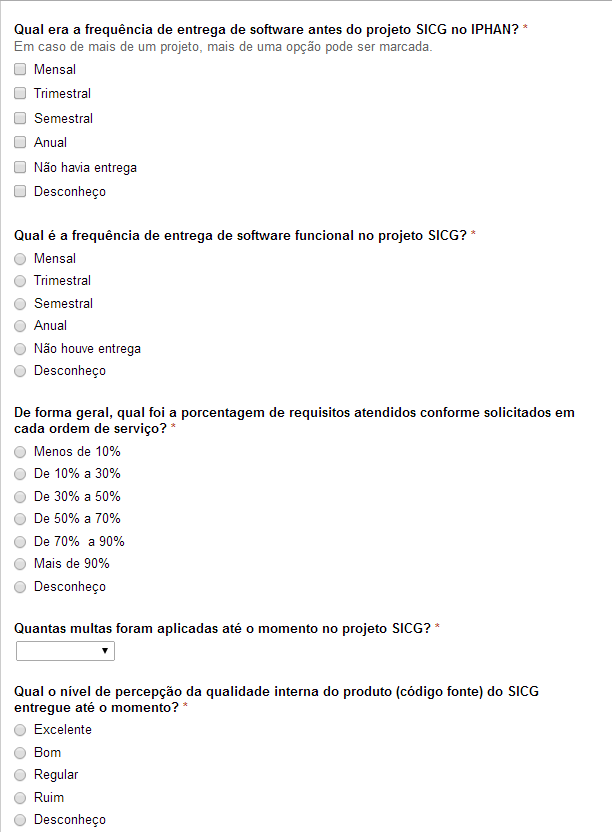
\includegraphics[scale=1.0]{figuras/quest6.png}

		\label{quest6}
\end{figure}

\begin{figure}[H]
		\centering
			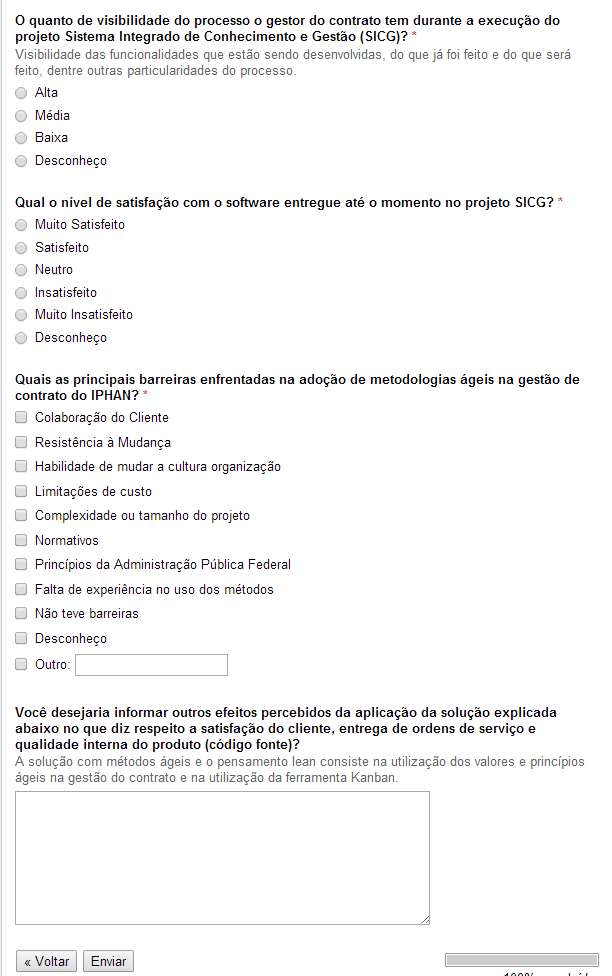
\includegraphics[scale=1.0]{figuras/quest7.png}

		\label{quest7}
\end{figure}

\chapter{Métricas de Código Fonte}

Neste trabalho foram selecionadas doze métricas de código fonte levantadas e categorizadas por \citeonline{Meirelles2013}: métricas de tamanho e complexidade e métricas de orientação à objetos.

As métricas de tamanho e complexidade selecionadas foram: 

\textbf{LOC (Lines of Code):} número de Linhas de Código foi uma das primeiras métricas
utilizadas para medir o tamanho de um software. São contadas apenas as linhas
executáveis, ou seja, são excluídas linhas em branco e comentários \cite{Jones91}.

 \vspace{\onelineskip} 

\textbf{ACCM (Average Cyclomatic Complexity per Method):} média da Complexidade
Ciclomática por Método mede a complexidade dos métodos ou funções
de um programa. Essa métrica pode ser representada através de um grafo de fluxo
de controle \cite{McCabe76}. O uso de estruturas de controle, tais como, if, else,
while aumentam a complexidade ciclomática de um método.

 \vspace{\onelineskip}

\textbf{AMLOC (Average Method Lines of Code)} - essa medida indica se o código está bem distribuído entre os métodos. Quanto maior, mais pesados são os métodos. É preferível ter muitas operações pequenas e de fácil entendimento que poucas operações grandes e complexas \cite{Meirelles2013}.



 \vspace{\onelineskip} 

As métricas de orientação à objetos selecionadas foram:

\textbf{ACC (Afferent Connections per Class):} conexões Aferentes por Classe é o número
total de classes externas de um pacote que dependem de classes de dentro desse
pacote. Quando calculada no nível da classe, essa medida também é conhecida como
Fan-in da classe, medindo o número de classes das quais a classe é derivada e, assim,
valores elevados indicam uso excessivo de herança múltipla \cite{McCabe94} \cite{Chidamber94}.

 \vspace{\onelineskip} 

 \textbf{ANPM (Average Number of Parameters per Method):}  calcula a média de parâmetros dos métodos da classe. Seu valor mínimo é zero e não existe um limite máximo para o seu resultado, mas um número alto de parâmetros pode indicar que um método pode ter mais uma responsabilidade \cite{Basili1987}


 \vspace{\onelineskip} 

\textbf{CBO (Coupling Between Objects):}   é o número total de classes dentro de um pacote que dependem de classes externas ao pacote. Quando calculada no nível da classe, essa medida também é conhecida como Fan-out da classe \cite{Chidamber94}

 \vspace{\onelineskip} 

\textbf{DIT (Depth of Inheritance Tree):} profundidade da Árvore de Herança é o número
de superclasses ou classes ancestrais da classe sendo analisada. São contabilizadas
apenas as superclasses do sistema, ou seja, as classes de bibliotecas não são
contabilizadas. Nos casos onde herança múltipla é permitida, considera-se o maior
caminho da classe até uma das raízes da hierarquia. Quanto maior for o valor DIT,
maior é o número de atributos e métodos herdados, e, portanto,maior é a complexidade
\cite{Shih97}.

 \vspace{\onelineskip} 

\textbf{LCOM4 (Lack of Cohesion in Methods):} falta de Coesão entre Métodos. Originalmente
proposto por \citeonline{Chidamber94} como LCOM não teve uma
grande aceitabilidade. Após críticas e sugestões a métrica foi revisada por \citeonline{LCOM4}, que propôs a LCOM4. Para calcular LCOM4 de um módulo, é
necessário construir um gráfico não-orientado em que os nós são os métodos e atributos
de uma classe. Para cada método, deve haver uma aresta entre ele e um outro
método ou variável que ele usa. O valor da LCOM4 é o número de componentes
fracamente conectados nesse gráfico.


 \vspace{\onelineskip} 

\textbf{NOC (Number of Children):} número de Filhos é o número de subclasses ou classes
filhas que herdam da classe analisada \cite{Rosenberg97}. Deve se ter
cautela ao modificar classes com muitos filhos, pois uma simples modificação de
assinatura de um método, pode criar uma mudança em muitas classes.


 \vspace{\onelineskip} 

\textbf{NOM (Number of Methods):} número de Métodos é usado para medir o tamanho
das classes em termos das suas operações implementadas. Essa métrica é usada para
ajudar a identificar o potencial de reúso de uma classe. Em geral, as classes com
um grande número de métodos são mais difíceis de serem reutilizadas, pois elas são
propensas a serem menos coesas \cite{Lorenz94}.


 \vspace{\onelineskip} 

\textbf{NPA (Number of Public Attributes):}  mede o encapsulamento. Os atributos de uma classe devem servir apenas às funcionalidades da própria classe. Portanto, boas práticas de programação recomendam que os atributos de uma classe devem ser manipulados através dos métodos de acesso \cite{beck1997smalltalk}



 \vspace{\onelineskip} 

\textbf{RFC (Response For a Class):} respostas para uma Classe é número de métodos
dentre todos os métodos que podem ser invocados em resposta a uma mensagem
enviada por um objeto de uma classe \cite{Sharble93}.



 \vspace{\onelineskip} 


\end{apendicesenv}
